\documentclass[11pt]{article}
% Project report. Numbers, tables and figures are filled in by analyze.py
% (results.tex, tests_table.tex, figures/). Edit the two macros below, then
% compile (Overleaf: upload report_overleaf.zip).

\newcommand{\authorNames}{Youssef Nassar}
\newcommand{\demoLink}{\textit{[add a link to your demo video here]}}

\usepackage[margin=1in]{geometry}
\usepackage{amsmath,amssymb}
\usepackage{graphicx}
\usepackage{booktabs}
\usepackage{xcolor}
\usepackage{listings}
\usepackage{caption}
\usepackage{tikz}
\usetikzlibrary{arrows.meta,positioning,fit}
\usepackage[hidelinks]{hyperref}

\definecolor{accent}{RGB}{42,120,214}
\lstset{basicstyle=\ttfamily\scriptsize, breaklines=true, frame=single,
        rulecolor=\color{black!25}, numbers=left, numberstyle=\tiny\color{black!45},
        keywordstyle=\color{accent}\bfseries, commentstyle=\color{black!55}\itshape,
        showstringspaces=false, columns=fullflexible, language=Python}

% ---- defaults, overwritten by results.tex once analyze.py has run ----
\newcommand{\pending}{\mbox{\textcolor{red}{[run analyze.py]}}}
\newcommand{\isSimulated}{0}
\newcommand{\runGain}{\pending}\newcommand{\runAtime}{\pending}\newcommand{\runSamples}{\pending}
\newcommand{\runMinutes}{\pending}\newcommand{\runMean}{\pending}\newcommand{\runMeanIR}{\pending}
\newcommand{\runSigma}{\pending}\newcommand{\runSigmaIR}{\pending}\newcommand{\runCorr}{\pending}
\newcommand{\runRawBits}{\pending}\newcommand{\runBits}{\pending}\newcommand{\runBytes}{\pending}
\newcommand{\runYield}{\pending}\newcommand{\runDice}{\pending}
\newcommand{\runFlicker}{\pending}\newcommand{\runVerdict}{\pending}
\IfFileExists{results.tex}{% generated by analyze.py - do not edit by hand
\renewcommand{\isSimulated}{0}
\renewcommand{\runGain}{MAX}
\renewcommand{\runAtime}{100}
\renewcommand{\runSamples}{2{,}608}
\renewcommand{\runMinutes}{5.0}
\renewcommand{\runMean}{10{,}826}
\renewcommand{\runMeanIR}{2{,}306}
\renewcommand{\runSigma}{1.56}
\renewcommand{\runSigmaIR}{0.74}
\renewcommand{\runCorr}{0.10}
\renewcommand{\runRawBits}{5{,}216}
\renewcommand{\runBits}{1{,}320}
\renewcommand{\runBytes}{165}
\renewcommand{\runYield}{25}
\renewcommand{\runDice}{4 2 2 1 3 2 2 5 2 5 5 3 6 3 3 1 6 6 3 1}
\renewcommand{\runFlicker}{The noise on the two photodiodes is nearly uncorrelated ($r=0.10$), so it is mostly independent per-diode noise (photon shot noise plus read noise) rather than flicker of the phone light, which would move both channels together.}
\renewcommand{\runVerdict}{The debiased stream passes all four tests at $\alpha=0.01$: no detectable bias or correlation in 1{,}320 bits.}
}{}

\newcommand{\fig}[3]{\IfFileExists{figures/#1}{\includegraphics[width=#2]{figures/#1}}%
  {\fbox{\parbox[c][4cm][c]{#3}{\centering figures/#1\\ \pending}}}}
\newcommand{\tbl}[1]{\IfFileExists{#1}{\input{#1}}{\pending}}
\newcommand{\code}[1]{\IfFileExists{code/#1}{\lstinputlisting[caption={\texttt{\detokenize{#1}}}]{code/#1}}{}}

\title{\textbf{Listening to Photon Noise}\\[4pt]
\large A low-voltage random-number generator and music machine from a light sensor}
\author{\authorNames}
\date{\today}

\begin{document}
\maketitle

\ifnum\isSimulated=1
\noindent\fcolorbox{red}{red!6}{\parbox{\dimexpr\linewidth-2\fboxsep-2\fboxrule}{\centering
\textbf{\textcolor{red}{SIMULATED DATA --- NOT A MEASUREMENT.}} These numbers come from
\texttt{--simulate}. Re-run \texttt{collect.py run} on the real sensor before submitting.}}
\medskip
\fi

\begin{abstract}
\noindent Light arrives in photons, so even a steady beam delivers a slightly different number of them
in every instant. We point a phone flashlight through a small paper-covered hole in a box onto a \$7, 3.3\,V light sensor
(ams TSL2591) read by a Raspberry Pi, record one \runMinutes-minute run, and use the last digit of each
reading as a source of random bits. A von Neumann extractor turns \runRawBits{} raw bits into \runBits{}
clean bits. \runVerdict{} The same bits drive live music in Sonic Pi. No high-voltage parts are used.
\end{abstract}

\section{Idea}
The original design counted single photons with a photomultiplier tube, which needs 500--1200\,V and a lab
safety review. This version uses a low-voltage integrating light sensor instead. It cannot see single
photons; it sums millions of them per 100\,ms reading. What it can see is the \emph{noise} on that sum,
and the last digit of a noisy number is hard to predict. That is enough to build a random-number
generator and to turn it into music. We do not claim a rigorous quantum random-number generator: the
noise is a mix of photon shot noise and electronic noise, and this build does not separate the two
precisely.

\section{Background}
\paragraph{Shot noise.} If photoelectrons arrive at random at a steady average rate, the number $N$
collected in one reading follows a Poisson distribution, with standard deviation $\sqrt{\langle N\rangle}$.
This fluctuation comes from the particle nature of light, not from the electronics.

\paragraph{Read noise.} The sensor's own amplifier and analog-to-digital converter add a few counts of noise
that are present even in the dark. Both kinds of noise are different on each of the TSL2591's two
photodiodes, whereas flicker of the light source moves both channels together. The correlation between the
two channels' noise therefore tells us whether the light source itself is the dominant noise.

\paragraph{From noise to bits.} When the noise is a few counts wide, the least-significant bit (LSB) of each
reading is close to a fair coin. A von Neumann extractor~\cite{vonneumann} removes remaining bias: bits are
read in pairs, $01\!\to\!0$, $10\!\to\!1$, and $00$, $11$ are discarded. It keeps about a quarter of the
bits. We check the result with four quick tests in the style of NIST SP~800-22~\cite{nist}.

\section{System}
\begin{figure}[h]
\centering
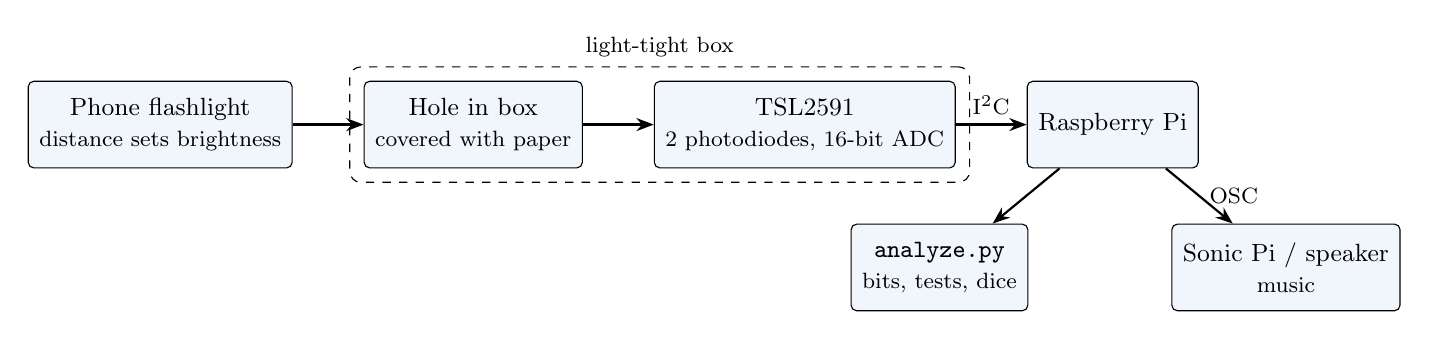
\begin{tikzpicture}[node distance=7mm and 9mm, font=\small,
  box/.style={draw, rounded corners=2pt, fill=accent!7, align=center, minimum height=11mm, inner sep=4pt},
  ar/.style={-{Stealth[length=2.2mm]}, thick}]
\node[box] (src) {Phone flashlight\\\footnotesize distance sets brightness};
\node[box, right=of src] (pin) {Hole in box\\\footnotesize covered with paper};
\node[box, right=of pin] (sen) {TSL2591\\\footnotesize 2 photodiodes, 16-bit ADC};
\node[box, right=of sen] (pi) {Raspberry Pi};
\node[box, below=of pi, xshift=-22mm] (ana) {\texttt{analyze.py}\\\footnotesize bits, tests, dice};
\node[box, below=of pi, xshift=22mm] (son) {Sonic Pi / speaker\\\footnotesize music};
\draw[ar] (src) -- (pin); \draw[ar] (pin) -- (sen);
\draw[ar] (sen) -- node[above]{\footnotesize I\textsuperscript{2}C} (pi);
\draw[ar] (pi) -- (ana); \draw[ar] (pi) -- node[right]{\footnotesize OSC} (son);
\node[draw, dashed, rounded corners, fit=(pin)(sen), inner sep=5pt, label={[font=\footnotesize]above:light-tight box}] {};
\end{tikzpicture}
\caption{Signal chain. Everything runs from the Pi's 3.3\,V rail.}
\end{figure}

\begin{table}[h]
\centering\small
\begin{tabular}{@{}ll@{}}
\toprule
Part & Role \\
\midrule
Adafruit TSL2591 breakout & two photodiodes (visible+IR, IR), 16-bit ADCs, I\textsuperscript{2}C at 0x29 \\
STEMMA QT cable & 3.3\,V, GND, SDA (GPIO2), SCL (GPIO3) to the Pi header \\
Opaque box, black foam tape & light-tight enclosure \\
Small hole in the box, printer paper over it & light entry and diffusion \\
Phone flashlight & light source; its distance sets the brightness \\
Raspberry Pi, USB speaker & acquisition, analysis, music \\
\bottomrule
\end{tabular}
\caption{Hardware used.}
\end{table}

\section{Method}
The sensor runs at gain \runGain{} (the highest) and \runAtime\,ms integration time. Each reading restarts the
converter and waits for a fresh result, so no reading is ever repeated. With paper taped over the
hole, the phone is moved until channel~0 reads between 3{,}000 and 25{,}000 counts (well above the dark
level, well below saturation), rested, and one run of \runSamples{} readings is recorded over \runMinutes\,min.

Noise is measured from sample-to-sample changes, $\sigma=\operatorname{std}(x_{i+1}-x_i)/\sqrt2$, which
ignores slow drift of the phone's light. The LSBs of both channels give \runRawBits{} raw bits, and von
Neumann extraction keeps \runBits{} of them (\runYield\,\%), saved as \runBytes{} bytes. For dice, clean bits
are read three at a time (0--7) and values 6 and 7 are discarded, so every face stays equally likely.

\paragraph{Music.} Every four clean bits make a note: three bits choose one of eight notes of A minor
pentatonic, one bit chooses a short or long decay. Notes go to Sonic Pi over OSC; the light level sets the
brightness of a background pad, so covering the hole darkens the sound. The same bits also drive a
Karplus--Strong plucked-string synthesizer and golden-ratio FM bells rendered to the USB speaker.
Demo: \demoLink.

\section{Results}
\begin{figure}[h]
\centering
\fig{noise.png}{0.74\linewidth}{0.6\linewidth}\hfill\fig{bits.png}{0.22\linewidth}{0.2\linewidth}
\caption{Left: first 60\,s of the run and the distribution of its sample-to-sample changes, with a
Gaussian of equal width. Right: the first clean bits as a black/white image; stripes or blocks would
reveal correlation.}
\end{figure}

Channel~0 averaged \runMean{} counts with noise $\sigma=\runSigma$ counts; channel~1 (IR) averaged
\runMeanIR{} counts with $\sigma=\runSigmaIR$ counts. \runFlicker

\begin{table}[h]
\centering\small\tbl{tests_table.tex}
\caption{Randomness tests; a test passes if $p\ge0.01$.}
\end{table}

\textbf{\runVerdict} The first dice rolls generated from the sensor noise: \textbf{\runDice}.

\section{Discussion}
\paragraph{What this shows.} A cheap light sensor's noise is wide enough that its last digit behaves like a
coin flip, and after debiasing the bits show no detectable bias or pattern at this sample size. Photon shot
noise is part of that noise, which is why covering the hole changes it.

\paragraph{Limitations.} (1) The sensor integrates millions of photons, so single photons are never seen.
(2) One run at one brightness cannot separate shot noise from read noise; measuring the noise at several
distances and checking that the noise variance grows in proportion to the signal would. (3) Four quick tests
on about a thousand bits catch obvious flaws only; a real random-number generator needs the full NIST suite
on millions of bits. (4) The phone flashlight may flicker; the two-channel correlation above flags this.

\paragraph{Next steps.} Record at several phone distances to measure the shot-noise fraction; run longer to
collect enough bits for the full NIST suite; replace the sensor with a single-photon detector once a
high-voltage safety review is possible.

\section{Conclusion}
A \$7 light sensor, a box with a paper-covered hole, a phone flashlight and a Raspberry Pi make a working low-voltage random
number generator whose output you can hear.

\begin{thebibliography}{9}
\bibitem{vonneumann} J.~von Neumann, ``Various techniques used in connection with random digits,''
  \emph{NBS Applied Mathematics Series} 12, pp.~36--38, 1951.
\bibitem{nist} A.~Rukhin \emph{et al.}, \emph{A Statistical Test Suite for Random and Pseudorandom
  Number Generators}, NIST SP~800-22 Rev.~1a, 2010.
\bibitem{tsl} ams AG, \emph{TSL2591 Light-to-Digital Converter}, datasheet.
\bibitem{sonicpi} S.~Aaron, \emph{Sonic Pi}, \url{https://sonic-pi.net}.
\end{thebibliography}

\appendix
\section{Code}
\code{sensor.py}
\code{collect.py}
\code{analyze.py}
\code{sonify.py}
\code{waves.py}
\lstset{language={}}
\code{sonic_pi.rb}

\end{document}
